\documentclass[a4paper]{article}



%% Language and font encodings
\usepackage[english,spanish]{babel}
\usepackage[utf8x]{inputenc}
\usepackage[T1]{fontenc}

\usepackage{hyperref}
\usepackage{caption}
\usepackage{subcaption}
\usepackage{booktabs}



%% Sets page size and margins
\usepackage[a4paper,top=3cm,bottom=2cm,left=3cm,right=3cm,marginparwidth=1.75cm]{geometry}
%% para subrayar, colores, bold, etc
\usepackage{color,soul}
%% Useful packages
\usepackage{amsmath}
\usepackage{graphicx}
\usepackage{float}
\usepackage[colorinlistoftodos]{todonotes}



\begin{document}

\title{%

\includegraphics[scale = 0.5]{./header_unc.png}\\[1.0 cm]	% University Logo
  Practica Profesional Supervisada\\
  \large Ingeniería en Computación FCEFyN - UNC
  }


  \author{ Casabella Martin, 39694763\\
			Sulca Sergio, xxxxxxxx\\
			Vignolles Ivan Maximiliano, xxxxxxxx
}
\clearpage
\maketitle

\section*{Objetivo} \label{objetivo_sec}
El objetivo de la Práctica Profesional Supervisada, en adelante PPS, es lograr la inserción laboral del alumno en la realidad profesional del país, en el área que mejor responda a sus aspiraciones profesionales e intereses vocacionales, con el propósito de fortalecer su formación académica y de establecer un vínculo que facilite su ingreso como profesional al mercado de trabajo. 
Este proyecto consta en el diseño e implementación en una FPGA (Field Programmable Gate Array) de un sistema destinado al procesamiento digital de imágenes vía hardware. 
Fue desarrollado en la institución Fulgor, bajo la supervisión del Dr.Ing. Ariel Luis Pola.

\section*{Motivación}  \label{motiv_sec}
El filtrado y procesamiento de imágenes es utilizado en múltiples campos, como la medicina, ingeniería, navegación, aeronáutica, entre otros. En el campo de la inteligencia artificial, área emergente que es de mero interés hoy en día, la convolución en 2D es la operación principal que se realiza durante el feed forward de una CNN (Red neuronal Convolucional). 
Dada su naturaleza, la operación de convolución en 2-D es la más empleada en los algoritmos de procesamiento de imágenes. El paralelismo inherente de algoritmos basados en la convolución es explotado logrando alta performance en estos sistemas que los utilizan.
El uso de Field Programmable Gate Arrays (FPGAs) para implementar este tipo de sistemas, se debe a la ventaja que presentan estos dispositivos en lo que concierne al paralelismo a nivel bit, pixel, vecindad y a nivel tarea, lo incrementa la performance y velocidad de cómputo.
Se presenta una arquitectura para la implementación en hardware de la operación de convolución 2-D priorizando el uso eficiente de recursos junto con la escalabilidad del diseño y velocidad de procesamiento.



\section{Introducción al proyecto} \label{intro_secc}
\subsection{Representación en punto fijo y cambio de rango dinámico }\label{fixedpoint}
La convolucion bidimensional, se define matemáticamente como:
\begin{equation}\label{conv-org}
  G(x,y) = \sum_{i=0}^{m-1} \sum_{j=0}^{n-1}K(i,j)I(x-i,y-j)
\end{equation}
Donde $I(x,y)$ es una imagen de $(m \times n)$ pixels, $K(i,j)$ un conjunto de coeficientes denominado kernel, de tamaño
$(k \times k)$ and $G(x,y)$ es la convolucion resultante de tamaño  $(m-2 \times n-2)$ .\\

\underline{\textbf{Representación en punto fijo:}}

La representación en punto flotante, almacena los números en términos de la mantisa y del exponente. El hardware que soporta el formato punto flotante, luego de ejecutar cada computo, 
automáticamente escala la mantisa y actualiza el exponente para que el resultado se corresponda con el número de bits de forma definida. Todas estas operaciones hacen que el hardware que soporte punto flotante,
sea más costoso en términos de área y potencia. Emerge una alternativa: la representación en punto fijo.
Este formato se emplea para almacenar y manipular datos, con cierto número de bits fijos. Esto implica que luego del cómputo, no se sigue la posición del punto decimal, y
se le delega esta responsabilidad al diseñador del hardware. El punto decimal, valga la redundancia, es fijo para cada variable, y es predefinido.
Fijando el punto, una variable se limita a tomar un rango fijo de valores.
Pese a que este límite nos brinda ventajas en lo que refiere a utilización de recursos, si el resultado del cómputo cae fuera del rango, se produce un overflow. Existen varias
formas de manipular los overflows que emergen como resultado de un cómputo en punto fijo (redondeo, saturación, truncamiento) y sigue siendo responsabilidad del diseñador optar por
la representación adecuada según el sistema que pretende llevar a cabo.

FALTA:    QUE REPRESENTACION USAMOS Y  PORQUE (GRAFICOS). NO LO PUSE PORQUE NO SE CON CUAL NOS QUEDAMOS AL FINAL

\subsection{Expansión dinámica de rango y Maximun Norm}\label{dynamicrange}
Los pixeles de la imagen en escala de grises $I(x,y)$ tienen un rango dinámico de valores que se hallan entre $[0,255]$,
y los valores que toma el kernel $K(x,y)$ pueden ser positivos o negativos.\\
Dado que el sistema desarrollado forma parte de un proyecto de Deep Learning, donde es usual operar en un rango dinámico centrado en cero, se aplicó una transformación denominada  expansión dinámica de rango ( $\mathcal{D}[.])$ ),
junto con Maximun Norm ($(\mathcal{M}[.])$) para reacomodar los diferentes rangos de valores.

Para el caso de la imagen, se tiene $\mathcal{D}[I(x,y)]=I^\prime(x,y)$ y un rango resultante de $[0,1]$.
Para el caso del kernel, $\mathcal{M}[K(x,y)]=K^\prime(x,y)$ con un rango $[-1,1]$, respectivamente.
Asi, reemplazando en ~\eqref{conv-org}, se tiene 

\begin{equation}\label{conv-org1}
  G(x,y) = \mathcal{D}^{-1}\left[\sum_{i=0}^{m-1} \sum_{j=0}^{n-1}K^\prime(i,j)I^\prime(x-i,y-j)\right],
\end{equation}\\
siendo $\mathcal{D}^{-1}[.]$ el cambio de rango dinamico entre $[0,255]$ en la FPGA.

\begin{figure}[H]
\centering
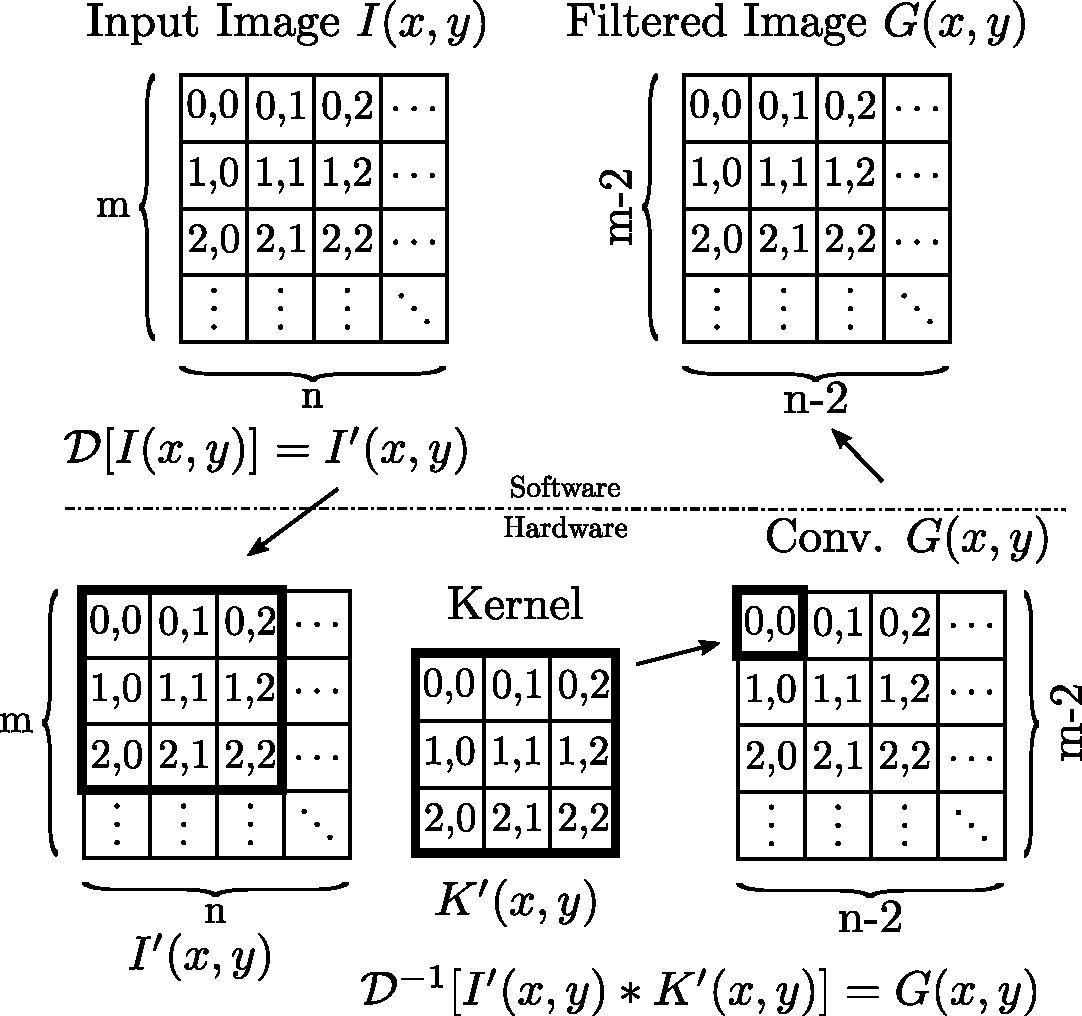
\includegraphics[scale=0.47]{wflow3}
\caption{Transformaciones del rango dinámico durante el procesamiento de la imagen.}
\label{transformation}
\end{figure}

\subsection{Flujo de diseño} \label{flujo_subsecc}
Se estructuró el proyecto y se siguió el siguiente flujo o estructura para llevarlo a cabo en el tiempo disponible\\

\begin{figure}[H]
\centering
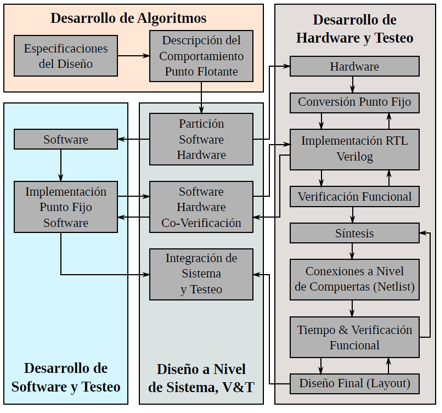
\includegraphics{flujo_de_dis.png}
\caption{Esquemático del flujo de diseño seguido.}
\label{design_flow}
\end{figure}

En primera instancia se partió de las especificaciones, simulando el comportamiento en punto flotante mediante el lenguaje de alto nivel Python. Luego, se analizaron los resultados obtenidos tras implementar el sistema en punto fijo, a nivel software. 
Fijados los requerimientos se comenzó con la programación del hardware, previamente habiendo estudiado y modelado la arquitectura del sistema, la cual se detallará posteriormente. \\\\


Como instancias intermedias se realizaron diferentes tipos de testing: test unitarios de cada módulo (test bench del módulo), test de integración (varios módulos y su interacción) y finalmente test de sistema, donde se probó el funcionamiento del sistema completo dada cierta imagen de entrada.

\begin{figure}[H]
\centering
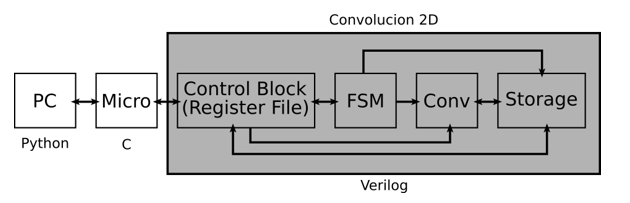
\includegraphics{general_sch.png}
\caption{Diagrama general del sistema: comunicación y lenguajes empleados.}
\label{design_flow}
\end{figure}

\section{Arquitectura del sistema}  \label{arquitectura_sec}
\subsection{Flujo de trabajo}  \label{workflow_subsecc}

Describiremos el diseño confeccionado en detalle. Se tienen tres etapas fundamentales:


\begin{frame}{}

    
      \begin{itemize}
        \item \textbf{Pre-procesamiento:} consiste en capturar la imagen aplicando las transformaciones mencionadas en la sección \ref{fixedpoint}, empleando un script hecho en Python. Este script divide la imagen en lotes o batches y los envía a la FPGA, a través del puerto UART. Un batch o lote, consiste en columnas contiguas de pixeles cuya dimensión se explica en la sección x.
%%Poner seccion aca
        \item \textbf{Procesamiento:}	: el batch es convolucionado con el kernel dentro del módulo. Dicho kernel es configurable, y el usuario puede cargar los coeficientes del mismo mediante el GPIO. 
Cuando la operación de la convolucion finaliza, una notificación es enviada al microprocesador, que da la orden de recuperar el batch procesado, para así enviarlo a la unidad central de procesamiento (CPU).
       \item \textbf{Post-procesamiento:}Como etapa final, en el post-procesamiento se combinan los batches o lotes en CPU usando el script de Python.
      \end{itemize}
     
\end{frame}


Se anexa el diagrama de estados del sistema, para procesar cierta imagen de entrada dada:\\

\begin{figure}[H]
\centering
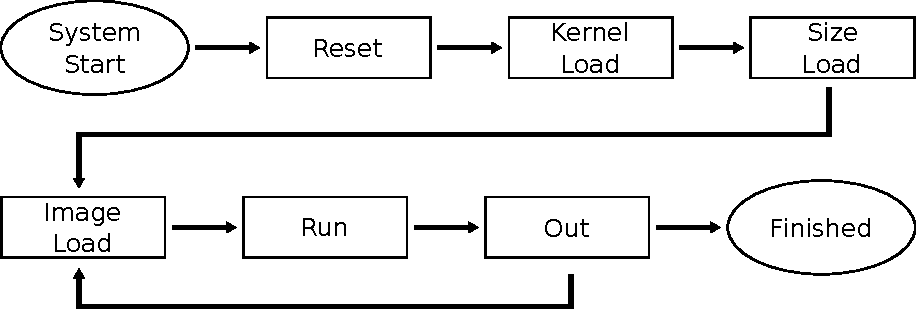
\includegraphics[scale=0.7]{states.pdf}
\caption{Diagrama de estados del sistema.}
\label{statesfig}
\end{figure}

\subsubsection{Estados y transiciones}  \label{states_subsecc}

La transición entre un estado y otro se realiza mediante instrucciones codificadas en el frame de entrada de 32 bits asentado en el GPIO. El modulo permanece en su estado actual hasta recibir una instrucción valida.

Inicialmente, debe situarse al sistema en un estado de reset, y por ende debe recibir dicha señal de reset para establecerse en dicho estado, esperando a ser configurado.
Luego de recibir la correspondiente instrucción, se produce una transición hacia el estado KernelLoad, en donde los coeficientes del kernel se cargan al módulo.
El siguiente estado (SizeLoad), es en el cual se carga el tamaño de la imagen, más precisamente la altura de la misma o el número de filas de las BRAM a ser instanciadas.
Estos tres estados mencionados, solo se ejecutan una vez durante todo el ciclo de trabajo. El proceso se repite por cada nueva imagen, por ende, si se desea procesar una nueva imagen, inicia el ciclo nuevamente.\\


Arrancando con el procesamiento de los lotes, primero la transición es hacia el estado ImageLoad, donde se almacena el lote en la Block RAM de la FPGA. 
Teniendo el lote almacenado, la transición luego es hacia el estado run donde se hace el procesamiento en si, y mientras el sistema se situe en este estado, no puede ser interrumpido. \\


Como consecuencia, cualquier instrucción recibida se ignora hasta que se complete esta etapa de procesamiento de lote.
Cuando se finaliza el procesamiento de un lote, se emite una notificación hacia el pin EoP (End Of Process) de la unidad de control (Control Unit), y el sistema espera a la última transición hacia el estado Out. Ni bien recibe la correspondiente instrucción codificada, se devuelve el lote procesado al microprocesador de la PC.

\begin{figure}[H]
\centering
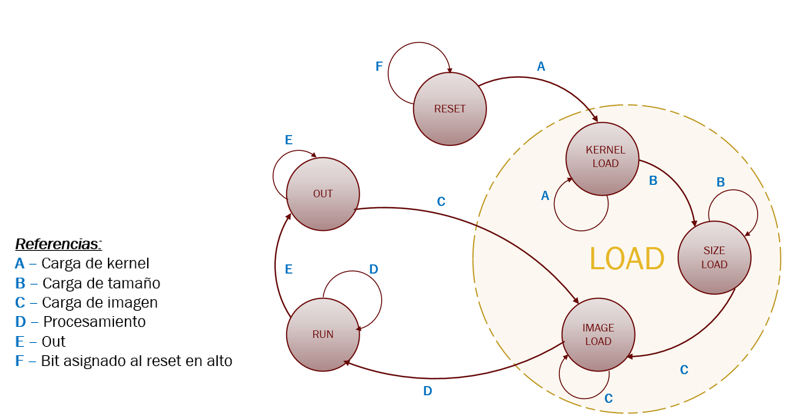
\includegraphics{states_2.png}
\caption{Diferentes estados y las etapas involucradas }
\label{statesfig2}
\end{figure}

\subsection{Arquitectura propuesta}  \label{ourdesign_subsecs}


El diseño planteado prioriza la reutilización dinámica de memoria, en donde por cada iteración en la etapa de procesamiento, se aprovecha la disponibilidad de datos cargados en memoria en la iteración anterior. 
En el diagrama en bloques anexado en la parte superior, se muestran los bloques principales que conforman el diseño:

\begin{frame}{}

    
      \begin{itemize}
        \item \textbf{Control Unit:} se encarga del manejo de la comunicación entre el procesador
         \item \textbf{MAC Unit -Multiplier-ACcumulator:} ejecuta la suma de los productos entre los coeficientes del kernel y los pixeles de la imagen. 
        \item \textbf{Address Generation Unit (AGU):} modulo que maneja las direcciones de memoria que deben ser leídas o escritas
       \item \textbf{Storage:} hace referencia a un conjunto de columnas almacenadas en block RAMs de la FPGA. El tamaño se explicara posteriormente con detalle, ya que depende de la cantidad de MACs instanciadas, o en otras palabras, el paralelismo a nivel de cantidad de convoluciones en paralelo, que se desee en el sistema.

      \end{itemize}
     
\end{frame}
	

\begin{figure}[H]
\centering
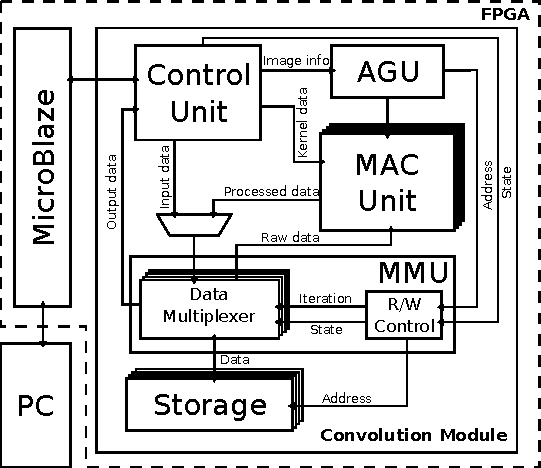
\includegraphics{general_architecture}
\caption{Arquitectura general del sistema }
\label{statesfig2}
\end{figure}

\subsubsection{Almacenamiento}  \label{storage_subsecc}
Los coeficientes del kernel se almacenan en registros dentro de cada MAC Unit. Para almacenar un lote, el enfoque que se opto fue organizar la BRAM en columnas. Cada columna entonces, corresponde a una columna del lote.
El tamaño del lote está dado por la altura de la imagen y por el número de columnas de memoria instanciadas.  La máxima altura de la imagen, entonces, debe ser menor o igual a la altura de la memoria instanciada.
Durante el procesamiento del lote, cada pixel se lee únicamente una vez, lo que permite un uso mas eficiente de la memoria. Los pixeles que ya se utilizaron, se sobrescriben con los pixeles procesados. 
Esto permite reducir la cantidad de memoria necesaria, ya que reúsa la misma memoria para almacenar el lote de entrada, y el lote procesado.

\subsubsection{Procesamiento de datos}  \label{processing_subsecc}
Para un kernel de  $(k \times k)$, cada MAC Unit toma $k$ columnas de memoria adyacentes como entrada.\\

El bloque $MAC$  $Unit$ necesita primero que se carguen k pixeles de cada columna para asi tener $(k \times k)$ pixeles cargados dentro de ella para así producir el primer pixel procesado.\\

Luego, se procede a efectuar la multiplicación de los pixeles con los coeficientes del kernel y sumar cada termino.\\

Finalmente se trunca el resultado, y se almacena el mismo en la primera posición de memoria.\\

Una vez que se procesa un pixel, se almacena en la memoria mientras bloque $MAC$  $Unit$ efectua un desplazamiento (shift) de sus registros en donde se almacenan pixeles de la imagen, para asi descartar los k pixeles mas antiguos,
 y se cargan los $k$ nuevos pixeles, es decir, uno de cada columna de entrada, lo que es equivalente a una estructura FIFO (First Input – First Output).
Se sincroniza lo mencionado anteriormente de forma tal de obtener un pixel por cada ciclo de clock.\\

Este procedimiento es equivalente a desplazar verticalmente el kernel sobre la imagen:

\begin{figure}[H]
\centering
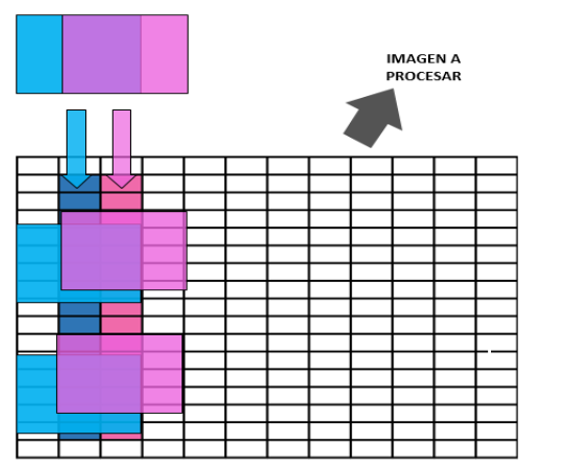
\includegraphics[scale=0.7]{conv1_despl.png}
\caption{Desplazamiento vertical del kernel sobre la imagen }
\label{verticaldesp}
\end{figure}


El módulo $AGU$ maneja las direcciones de memoria, tanto lectura como de escritura, teniendo en cuenta la latencia desde que un pixel se carga en bloque $MAC$ $Unit$ hasta que el pixel procesado correspondiente sea almacenado.
Todo lo mencionado anteriormente fue de manera genérica sobre una sola MAC Unit, pero ahora se explicara como poder trabajar en el sistema con mas de uno de estos modulos instanciados en paralelo:
\begin{frame}{}

    
      \begin{itemize}

\item Como se mencionó,  se necesitan $k$ columnas como entrada para producir una columna procesada en una $MAC$ $Unit$. Por lo tanto, $2 \times k$ columnas, se necesitan para $2$ $MACs$.
\item Debido a la naturaleza de la operación de la convolucion, para obtener una columna contigua, se necesita desplazar una vez las columnas de entrada. Entonces, existe un solapamiento entre 2 de las entradas de las MACs que producen columnas adyacentes, y así la información puede ser compartida.
Así, pese a necesitar $k$ columnas de entrada por cada unidad $MAC$, solamente $k+1$ columnas diferentes de entrada se necesitan para dos $MACs$ instanciadas.
\item Entonces, para $N$ $MACs$, el número requerido de columnas de memoria, se reduce de $N \times k$ a $N+k-1$, concluyendo que agregar una nueva unidad $MAC$ solamente agrega una nueva columna de memoria.
\item Debido al solapamiento explicado anteriormente, hay información repetida entre un lote recibido y el siguiente, por lo que, para reducir la transmisión de datos, esta información repetida se mantiene en memoria y solamente se transmite la parte faltante del lote entrante.
Dadas $N$ $MACs$ y  un kernel de $k \times k$, un lote cuyo ancho (o cantidad de columnas) sea de $N+k-1$ es necesario. No obstante, el lote procesado tendrá un ancho de  $N$ columnas, es decir, una por unidad $MAC$, por lo que las ultimas $k+1$ memorias no se sobrescriben y mantienen los datos de entrada. Estas $k+1$ columnas se reutilizan como las primeras columnas del siguiente lote, y asi, el ancho del lote transmitido se reduce a $N$, con la excepción de que el primer lote mantiene un ancho de $N+k-1$.

      \end{itemize}
     
\end{frame}


La reutilización de columnas de memoria escritas por los lotes previos, resulta en un desplazamiento circular en $N$ lugares, desplazando la posición de las columnas de memoria asociadas con cada unidad $MAC$ en cada iteración.De lo anterior, se deduce que existe una periodicidad entre la relación de columnas de memoria y las entradas de las unidades $MAC$, donde el periodo It es el número de iteraciones necesario para obtener la relación ente las columnas de memoria originales con respecto a las entradas de las unidades $MAC$.
Entonces, matemáticamente: Cuando $It(k-1)$ es un múltiplo de $N+k-1$, debe existir un numero entero $m$, tal que:

\begin{equation}\label{niter}
  \frac{It}{m} = \frac{N}{k-1} + 1
\end{equation}

Sintetizando el algoritmo descrito, dadas $N$ $MACs$ y  un kernel de $ k \times k$:
\begin{frame}{}
	    
      \begin{itemize}

	\item Lote de imagen sin procesar,  con $N+k-1$ columnas es necesario
	\item El lote procesado tendrá un ancho de $N$ columnas
	\item Las ultimas $k+1$ memorias no se sobrescriben
	\item Estas $k+1$ columnas se reutilizan como las primeras columnas del siguiente lote
	\item El ancho del lote transmitido se reduce a $N$, con la excepción de que el primer lote mantiene un ancho de $N+k-1$.
	\item Sea el periodo $It$  el número de iteraciones necesario para obtener la relación ente las columnas de memoria originales con respecto a las entradas de las unidades $MAC$.
	\item Cuando $It(k-1)$ es un múltiplo de $N+k-1$, existe un numero entero $m$, tal que:
\begin{equation}\label{niter}
  \frac{It}{m} = \frac{N}{k-1} + 1
\end{equation}


\end{itemize}
\end{frame}

\bigskip
\bigskip
\bigskip

Veamos las ventajas del diseño planteado de forma gráfica:

\begin{figure}[H]
\centering
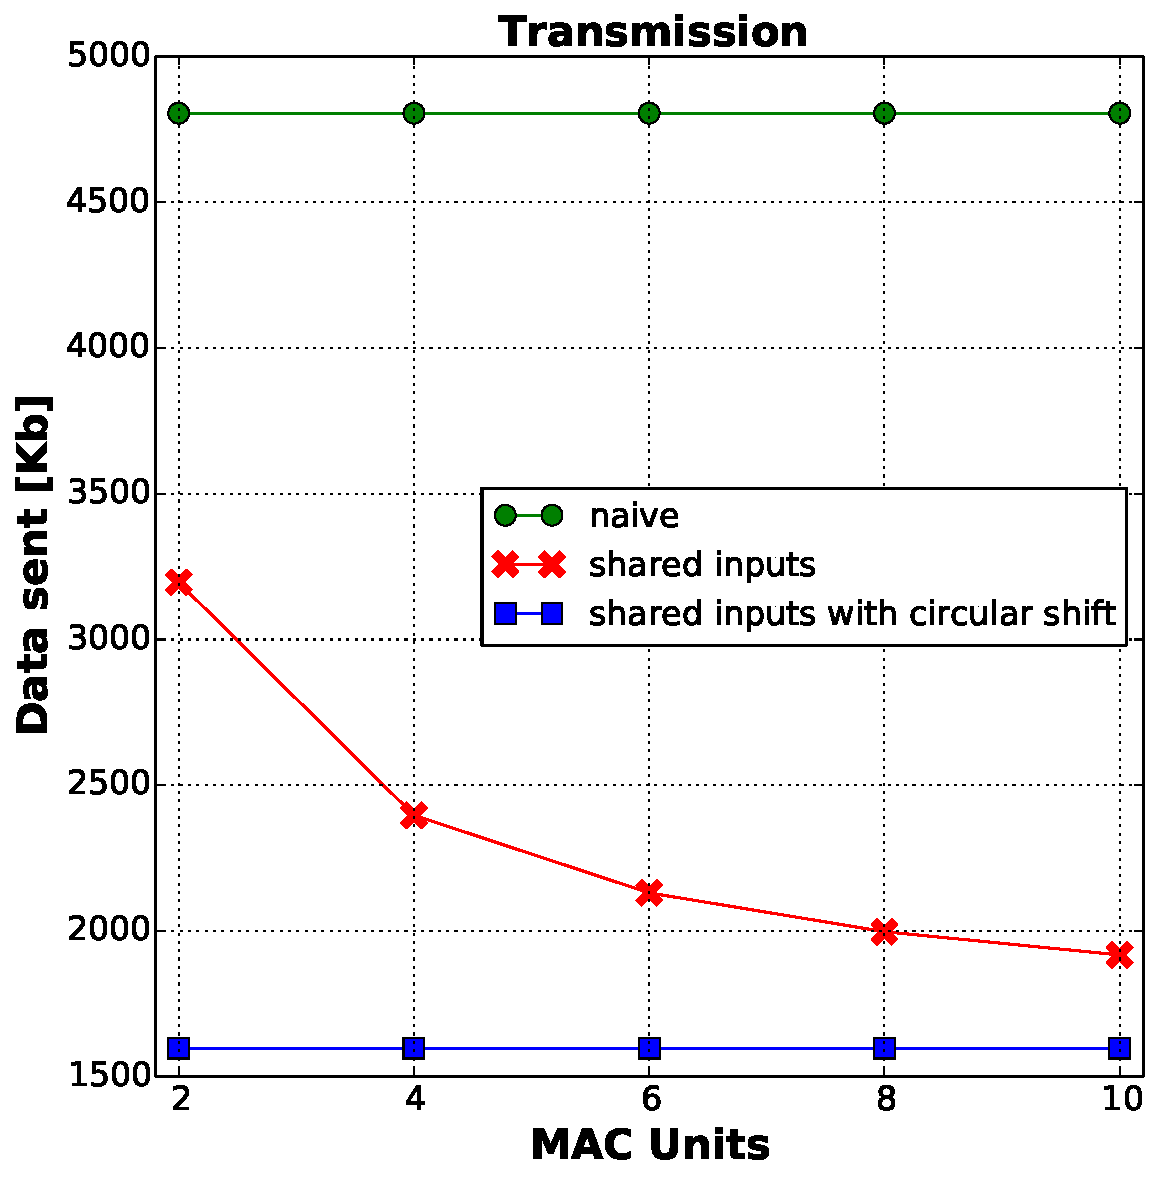
\includegraphics[scale=0.5]{data_sent}
\caption{Cantidad de memoria requerida en función del grado de paralelismo }
\label{memoryrequired}
\end{figure}

\bigskip
Se ve en la figura que a medida que se instancian más unidades $MAC$, o en otras palabras, a medida que se aumenta el grado de paralelismo del sistema haciendo referencia a la cantidad de convoluciones en paralelo con las que se trabaja, el primer enfoque propuesto requiere mucha mas memoria para operar que el enfoque de información compartida, donde se reutilizan ciertas columnas dada por la matemática y relaciones descritas.\\

\bigskip
\bigskip
Por otra parte, para lo que refiere a la transmisión, se tiene:

\begin{figure}[H]
\centering
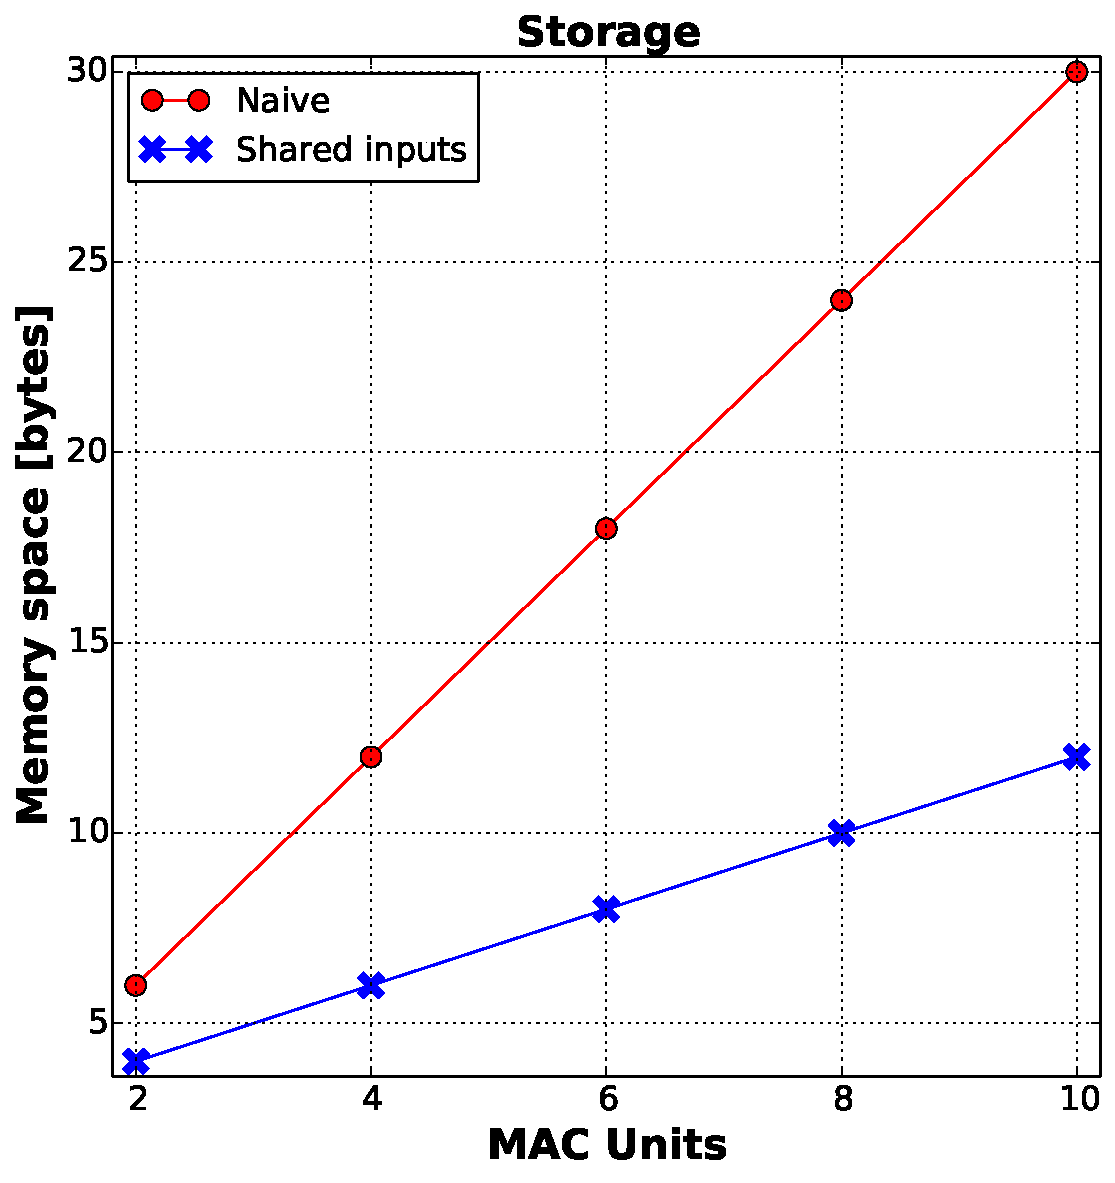
\includegraphics[scale=0.5]{mem_space2}
\caption{Transmisión de datos en función de unidades MAC instanciadas }
\label{datatransmision}
\end{figure}

Se mencionó que, debido al solapamiento, hay información repetida entre un lote recibido y el siguiente, por lo que, para reducir la transmisión de datos, esta información repetida se mantiene en memoria y solamente se transmite la parte faltante del lote entrante.\\

En la figura se muestra como el diseño planteado con el desplazamiento circular requiere una transmisión constante notablemente menor a comparación del primer enfoque que se planteo, y como también el hecho de reutilizar la información compartida tiende a una disminución en la transmisión de datos durante el funcionamiento del sistema. La imagen con la que se efectuaron las gráficas tenía un tamaño de $1600 \times 1024$.

\bigskip
\bigskip
\bigskip

\subsubsection{Proceso de escritura en memoria}  \label{writing_subsecc}
\smallskip
Se analiza el caso de tener instanciadas $N=4$, $MACs$ y un kernel con $k=3$ para clarificar la operación del algoritmo descrito.
El proceso de escritura en memoria, utilizando el desplazamiento circular de columnas mencionado.\\

Como consideramos un kernel con k=3 y s N=4, MACs:
\begin{frame}{}
	    
      \begin{itemize}
        \item Se necesitan o requieren N+k-1=4+3-1=6 columnas de memoria
	\item En la primera iteración, se cargan las memorias 1 a 6 con el nuevo lote (donde cada memoria instanciada alberga una columna del lote) y el resultado se almacena en las memorias 1 a 4, marcadas con otro color y en la etapa run  out.
	\item En la segunda iteración, los datos del nuevo lote se cargan sin sobrescribir las memorias 5 y 6 . Luego del procesamiento, se almacenan los datos comenzando en la memoria  5 hasta la última, para luego sobrescribir los datos del lote previo desde el principio.

\bigskip
\bigskip
Lo anterior se puede apreciar en la siguiente figura, donde se incluye una línea punteada que separa la etapa de carga y la de procesamiento y salida de dato:

\end{itemize}
\end{frame}

\begin{figure}[H]
\centering
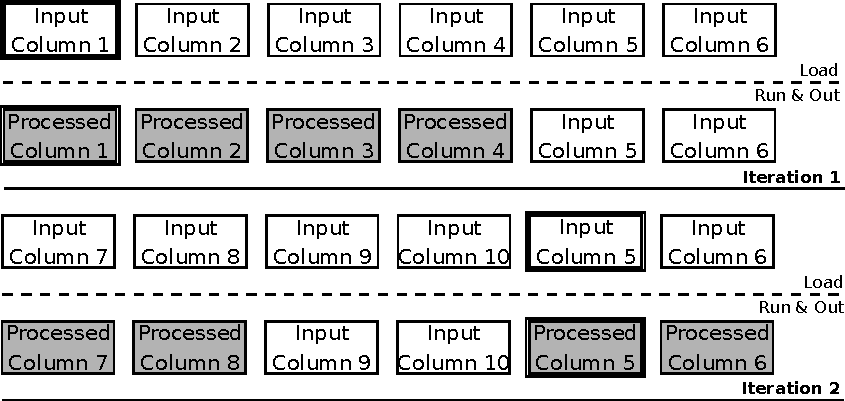
\includegraphics[scale=0.8]{algorithm}
\caption{Algoritmo de escritura para N=4, k=3 }
\label{writingprocess}
\end{figure}


La lógica del sistema se implementa en el bloque $MMU$ ($Memory$ $Managment$ $Unit$), que sirve como interfaz entre las memorias y el resto de los componentes, 
manteniéndolos independientes al grado de paralelismo del sistema y al número de iteración.

\bigskip

\subsection {MMU (Memory Managment Unit) }  \label{mmu_subsecc}
Este bloque, en cada iteración, mantiene un seguimiento de las posiciones de memoria donde el lote entrante debe ser almacenado,
la información que debe alimentar a cada unidad $MAC$, lLa posición de memoria donde la información procesada debe ser almacenada
y del orden en el cual la información procesada debe ser devuelta.

Para cumplir con estas funciones, se basa en una máquina de estados finitos interna al módulo, donde cada estado corresponde a un conjunto de las posiciones citadas anteriormente.
El número de estados está dado por el número de iteración de la ecuación:

\begin{equation}\label{niter}
  \frac{It}{m} = \frac{N}{k-1} + 1
\end{equation}

Este bloque consta de un conjunto de multiplexores cuyas líneas o entradas de selección son manejadas por la máquina de estados mencionada, para así hacer el routing de la información entrante y saliente, como se ve en la figura resaltado en color azul:
\begin{figure}[H]
\centering
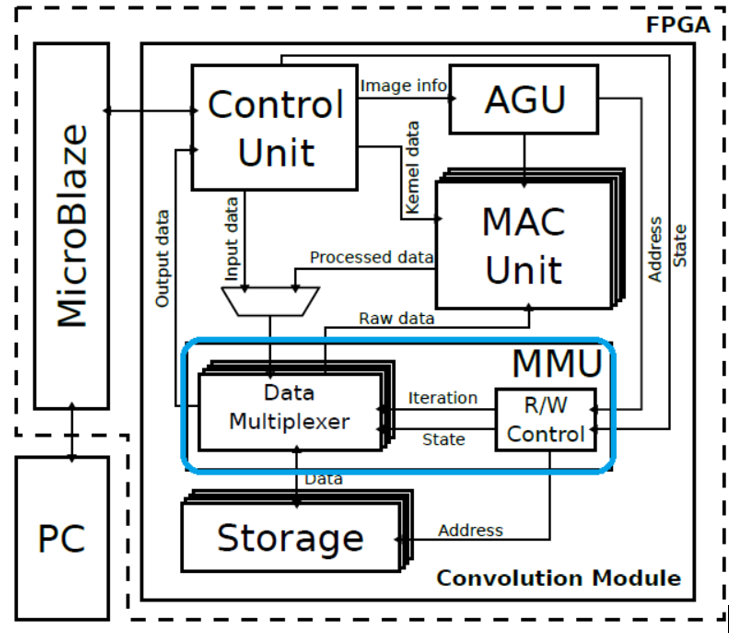
\includegraphics[scale=0.5]{arq_blue.png}
\caption{}
\label{mmu_location}
\end{figure}

Analizando la arquitectura interna de los bloques que conforman este módulo, el bloque data multiplexer está conformado por un conjunto de bloques más pequeños clasificados en dos clases acorde a la función que cumplen:
\begin{frame}{}
\begin{itemize}

 \item \textbf{$MMB$(Memory Multiplexer Blocks)}
  \item \textbf{$PMB$(Processing Multiplexer Blocks)}

\end{itemize}
\end{frame}


Los $MMB$ hacen el routing de la información sin procesar (raw data) y la información desde las unidades $MAC$ hacia las memorias.
Los $PMB$ hacen el routing de la información desde las memorias hacia las unidades $MAC$.\\

Este flujo se puede ver en la siguiente figura:
\begin{figure}[H]
\centering
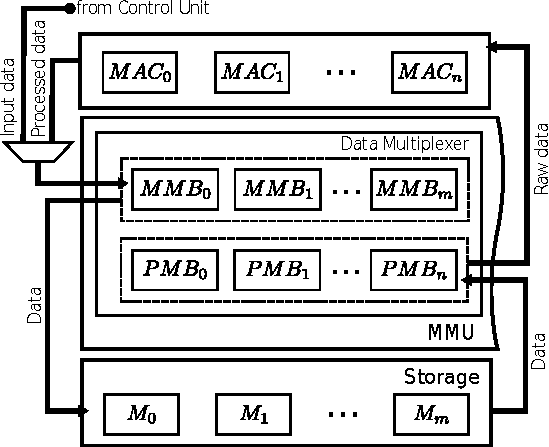
\includegraphics[scale=0.9]{muxes}
\caption{ Enrutamiento de información}
\label{mmu_routing}
\end{figure}
Tanto los bloques $MMB$ como los $PMB$ tienen un numero de entradas proporcional al numero de estados de la $FSM$ interna del bloque $MMU$. 
Las entradas a sus multiplexores se definen respectivamente:
\begin{equation}%\label{niter}
  O_j^i = O_{[(k-1)i+j]\%N}
\end{equation}
\begin{equation}%\label{niter}
  M_j^i = M_{(iN+j)\%(N+k-1)}
\end{equation}
\\
donde el símbolo $ \% $ representa la operación módulo, e $i$ toma valores desde $0$ a $It-1$.

\bigskip
\bigskip
\begin{figure}[H]
\centering
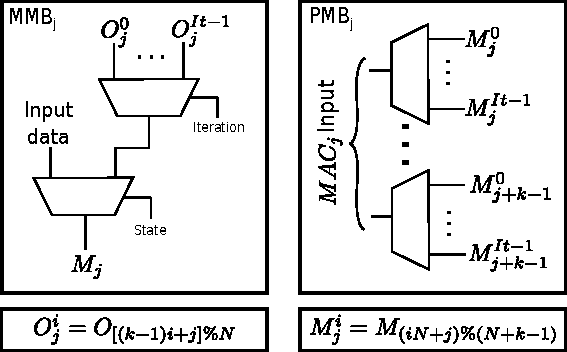
\includegraphics{muxes_cont}
\caption{ Estructura de los bloques MMB y PMB}
\label{mmu_structure}
\end{figure}


\section{Implementación y resultados}  \label{implementations_sec}
 diseño e implementación
El diseño fue implementado en una FPGA Xilinx Artix-35T (xc7a35ticsg324-1L) utilizando las herramientas del software
Xilinx Vivado Design Suite 2017.4. Se trabajó con un clock de referencia de $100$ MHz, y el script para el pre-procesamiento 
y el post-procesamiento fueron escritos en Python 2.7.

Tanto los coeficientes del kernel como el correspondiente lote de imagen, se cargan a la placa a través
del puerto UART. Si bien esta vía es lenta con respecto al tiempo de procesamiento, se optó por utilizarla
debido a su simplicidad y al bajo consumo de recursos comparado a otros medios de transmisión.

En lo que refiere a representación de datos, se trabajó con aritmética en punto fijo, con una
resolución de $U(8,0)$ para la imagen de entrada y salida (imagen procesada), y $S(8,7)$ para el kernel.


Para verificar el comportamiento del sistema. se armaron diferentes kernels
en Python, y se aplicaron los mismos a una imagen de prueba. Luego, 
se filtró a la imagen con los mismos kernels  pero utilizando la FPGA

Los kernels que se utilizaron fueron: identidad $[0, 0, 0; 0, 1, 0; 0, 0,
0]$ sharpening $[0, -1, 0; -1, 5, -1; 0, -1, 0]$ y embossing $[-2, -1, 0; -1,
0, 1; 0, 1, 2]$.\\


A la izquierda, se ve la imagen procesada con una $CPU$ utilizando Python, y a la derecha
la misma imagen filtrada en la placa:


\begin{figure}[H]
\centering
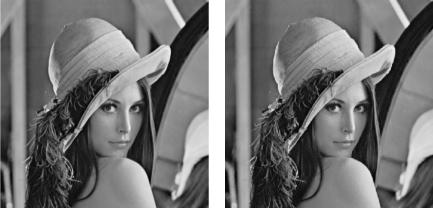
\includegraphics[scale=0.9]{identity_c}
\caption{Kernel Identidad}
\label{identity}
\end{figure}
\begin{figure}[H]
\centering
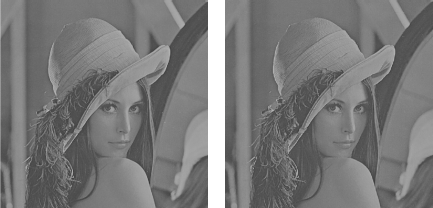
\includegraphics[scale=0.9]{shaped_c}
\caption{Sharpening Kernel}
\label{sharp}
\end{figure}

FALTA UNA QUE DICE TOO WIDE NOSE QUE MIERDA, Y NO LA SE PONER. TAMPOCO CON SUBFIG O SUBFLOAT, MUERTE A LATEX
\bigskip
\bigskip
\bigskip
\bigskip
\bigskip
\bigskip
\bigskip
\bigskip
\bigskip
\bigskip
\bigskip
\bigskip
\bigskip
\bigskip
\bigskip
\bigskip
\bigskip
\bigskip
\bigskip

%\begin{figure}[H]
%\centering
%\includegraphics[]{emboss2_c}
%\caption{Embossing Kernel}
%\label{emboss}
%\end{figure}




La arquitectura se sintetizó para diferentes grados de paralelismo.
La tabla Tabla~\ref{res_table} muestra la complejidad del modulo y el microprocesador en la FPGA
con y sin el uso de DSP respectivamente, medida por la utilización de recursos.
Se ve un incremento lineal acorde al grado de paralelismo en el sistema. Debido a las limitaciones de la FPGA utilizada,
se llegó a instanciar $8$ $MAC$ $units$ para que operen en pparalelo con DSP, y $24$ sin el uso de DSP pero con
una utilizacióon de $LUTs$ mas intensiva.

\begin{table}[H]
% increase table row spacing, adjust to taste
\renewcommand{\arraystretch}{1.3}
% if using array.sty, it might be a good idea to tweak the value of
% \extrarowheight as needed to properly center the text within the cells
\caption{Utilización de recursos con y sin DSP.}
\label{res_table}
\centering
% some packages, such as mdw tools, offer better commands for making tables
% than the plain latex2e tabular which is used here.
\begin{tabular}{|c|c|c|c|c|c|c|}
  \hline
  & \multicolumn{3}{c|}{\textbf{With DSP [N](\%)}} & \multicolumn{3}{c|}{\textbf{Without DSP [N](\%)}} \\ \hline
  \textbf{P}  & \textbf{DSP}            & \textbf{LUT}        & \textbf{BRAM}       & \textbf{DSP}         & \textbf{LUT}           & \textbf{BRAM}         \\ \hline
  2  & 20(22)         & 1845(9)    & 10(20)     & ---         & 3168(15)      & 10(20)         \\ \hline
  4  & 40(44)         & 2022(10)   & 11(22)     & ---         & 4627(22)      & 11(22)         \\ \hline
  6  & 60(67)         & 2175(10)   & 12(24)     & ---         & 6063(29)      & 12(24)         \\ \hline
  8  & 80(89)         & 2448(12)   & 13(26)     & ---         & 7756(37)      & 13(26)         \\ \hline
  10 & ---            & ---        & ---        & ---         & 9328(45)      & 14(28)         \\ \hline
  12 & ---            & ---        & ---        & ---         & 10917(52)     & 15(30)         \\ \hline
  24 & ---            & ---        & ---        & ---         & 20209(97)     & 21(42)         \\ \hline
\end{tabular}           
\end{table}



También se realizó una comparación entre la utilización de BRAM estmidada, y los resultados
obtenidos de la síntesis.\\

Se efectuó una normalización con respecto al porcentaje de utilización de BRAM dividiendo el máximo
valor de porcentaje de utilización, y considerando que la instancia del microblaze ya ocupa $18\%$
de los recursos BRAM. 
\begin{figure}[H]
\centering
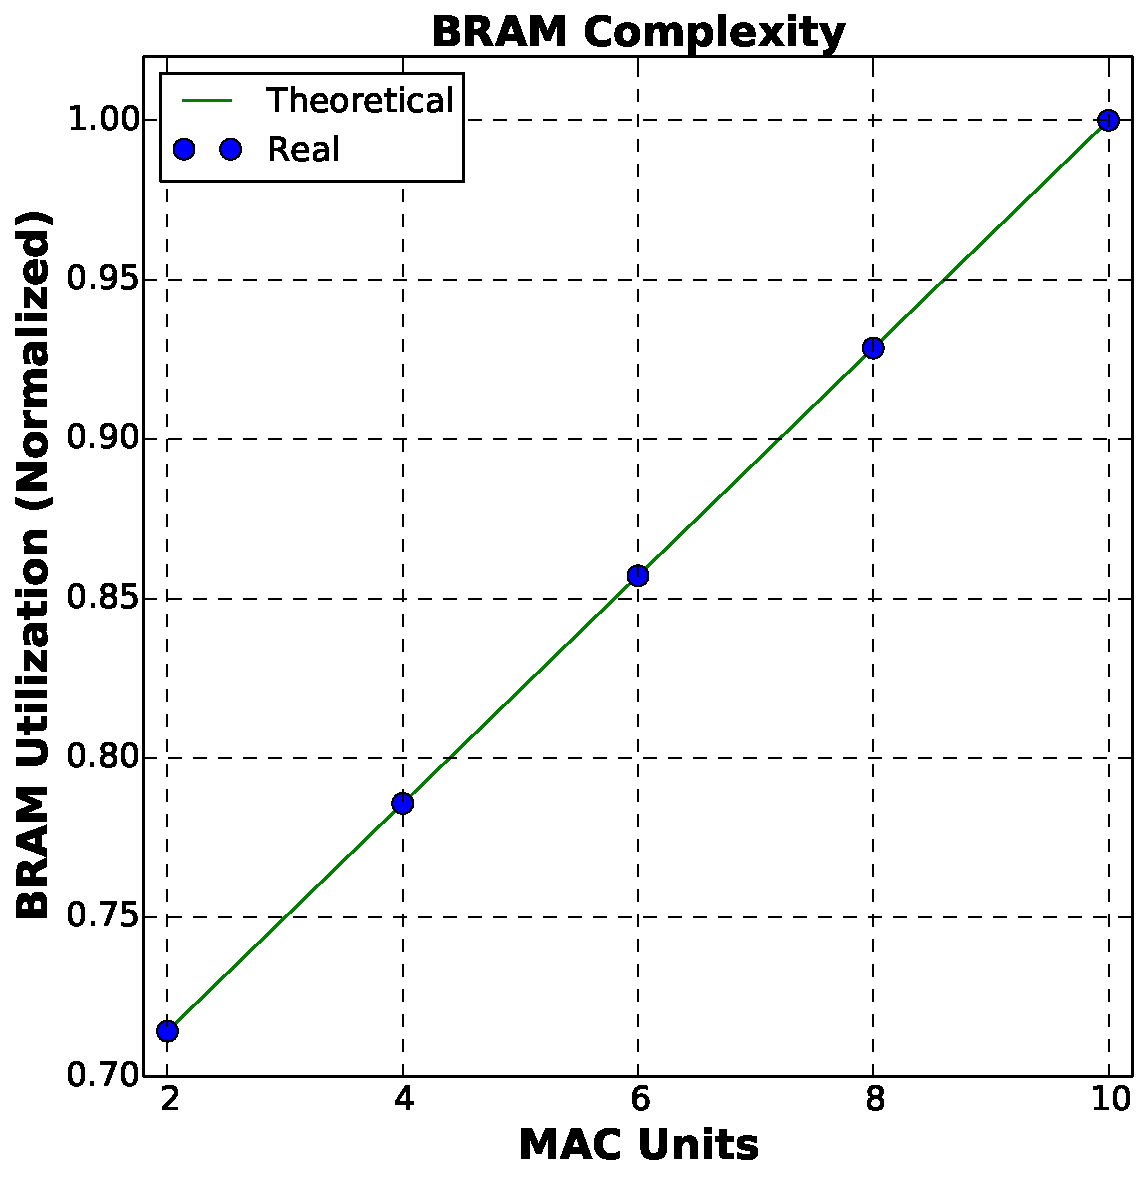
\includegraphics[scale=0.3]{BRAM_c2}
\caption{Normalized curve for BRAM resources utilization.}
\label{bram_n}
\end{figure}

Puede observarse que el comportamiento lineal anticipado por los
cálculos teóricos, es consistente con los resultados de la síntesis.\\


Considerando únicamente la operación de convolución, es decir, no teniendo en cuenta el tiempo
necesario para cargar la imagen en memoria, se obtiene un pixel por ciclo de clock ($100$ Mhz) por
cada $MAC$ $Unit$ instanciada.
\bigskip

El throughput incrementa linealmente con el grado de paralelismo. La tabla \ref{conv_tp} muestra el throughput
obtenido para los diferentes grados de paralelismo.

\begin{table}[H]
% increase table row spacing, adjust to taste
\renewcommand{\arraystretch}{1.3}
% if using array.sty, it might be a good idea to tweak the value of
% \extrarowheight as needed to properly center the text within the cells
\caption{Throughput obtenido en lo que respecta a la convolución.}
\label{conv_tp}
\centering
% some packages, such as mdw tools, offer better commands for making tables
% than the plain latex2e tabular which is used here.
\begin{tabular}{|c|c|c|}
 \hline
  \textbf{Parallelism}  &    \textbf{Processing Speed [Mp/s]}  \\ \hline
          2             &                     200              \\ \hline
          4             &                     400              \\ \hline
          8             &                     800              \\ \hline
\end{tabular}           
\end{table}


\section{Conclusión}  \label{conclusion_sec}

La flexibilidad y elevada potencia de cálculo de una FPGA permite que se pueda
procesar y filtrar el lote de imagen, al mismo tiempo que se está cargando el lote
actual. \\

Se diseñó y presentó una implementación de la operación de convolución bidimensional en una
plataforma Xilinx Artix 7 FPGA basada en eficiencia en la utilización de recursos y en el paralelismo del sistema.\\
Se implementaron todas las etapas necesarias, considerando la etapa de carga, procesamiento, y salida. Se
encontró una relación entre ciertos bloques instanciados, lo que permitió a nuestro sistema trabajar con diferentes
niveles de paralelismo.\\

Ademas, se optimizó la utilización de recursos de almacenamiento implementando un algoritmo para las
operaciones con memoria y para la sincronización de módulos.\\
Esto permitió con una parametrización total del sistema, lo que hace escalable a la arquitectura propuesta.
El desempeño del sistema y los resultados obtenidos muestran que la utilización de recursos relacionados con
Block RAMs incrementan de forma lineal, como se buscó.\\

En lo que refiere al procesamiento, se obtuvo un throughput elevado, por ende del factor limitante mencionado relacionado 
con la velocidad de transmisión del UART.





























\end{document}`